\documentclass[11pt]{article}
\usepackage[margin=1in]{geometry}
\usepackage{amsmath,amssymb,amsthm}
\usepackage{graphicx}
\usepackage{booktabs}
\usepackage{microtype}
\usepackage[hidelinks]{hyperref}
\usepackage[numbers,sort&compress]{natbib}
\usepackage{xcolor}
\newtheorem{theorem}{Theorem}
\newtheorem{proposition}{Proposition}
\newtheorem{definition}{Definition}
\newcommand{\germ}{\textsf{germline}}
\newcommand{\sys}{\textsf{system}}

\title{Germline Context: An Immutable Inherited Task Channel\\for Multi-Agent Language Model Systems}
\author{Ihor Tanyenkov\\EntroPi}
\date{November 2026 --- preprint, v0.2}

\begin{document}
\maketitle

\begin{abstract}
Multi-agent language model systems lose the task they were given as it is relayed from agent to agent. We show that the loss is not gradual erosion but \emph{brief collapse}: an agent hands its answer down instead of the specification, the rate of collapse rises with depth, and the collapse causes the downstream failures. In analogy with Weismann's germ plasm, we propose carrying only the \emph{genotype} of a task, the user's original statement verbatim plus a reasoning class and a hash, in an immutable channel, the germline, that every agent inherits at every depth and that no agent's experience can rewrite. We formalise chained relay as a Markov chain whose information about the original task can only fall and, under ergodic rewriting, falls to zero, whereas an anchored lineage keeps full information at every depth. Experiments with Qwen3-32B on tasks with programmatic checkers confirm the mechanism: chained retention falls to 0.61 over six hops and leaf success from 0.78 to 0.33, while under the same conditions no constraint loss was observed in any arm that carries the original verbatim. We report three predictions, written down before the runs, that failed, including that a repeated system prompt removes drift as well as the germline does. The germline's advantage lies elsewhere: an editable block never deleted a constraint but accreted interpretations, and none of the prompts we tested, including a barrier sentence naming the attack, stopped an untrained model from obeying a forged message that a constraint had been withdrawn (compliance 0.89--1.00 in every arm at two model sizes). Training the germline as a chat role on Qwen3-8B installed that priority within the tested conditions: compliance fell from 0.86 to 0 of 72 lineages, including 0 of 24 on a task family held out of training and 0 of 36 under six attack phrasings never seen, with no false positives in 612 unattacked restatements. Zero of 72 bounds the rate, it does not guarantee it. The same training degraded competence on the held-out family, from 0.28 to 0.19, because a templated verification checklist displaced reasoning; we report this as a negative result and describe the corrected recipe. The harness is standard-library Python with deterministic checkers.
\end{abstract}

\section{Introduction}

A multi-agent system built from language models delegates: a coordinating agent writes a brief, a worker reads it, works, and perhaps briefs another worker. Each hand-off re-derives the task from the previous agent's description. The user's original words are usually gone after the first hop, and what remains is each agent's reading of its parent's reading. Practitioners know the symptom: after a few levels of delegation the leaves are solving a subtly different problem than the one posed, constraints have been dropped, and ``helpful'' clarifications have hardened into requirements nobody asked for.

Weismann \citep{weismann1892} proposed that heredity passes through a germ plasm sealed off from the body: an organism's acquired adaptations, however useful, never flow back into what it transmits. That barrier is what lets a lineage remain the same kind of thing across generations while each individual adapts freely. Multi-agent language model systems have no such barrier. Each agent inherits its parent's working understanding of the task, adaptations included; the inheritance is Lamarckian. We use the biology as a frame and a source of names, not as a mechanism. The mechanism is the data processing inequality for chained relays and, for the part that turns out to require training, an explicit priority rule.

We make four contributions.
\begin{enumerate}
\item A definition of the \emph{germline} for agent systems (\S\ref{sec:germline}): an immutable, byte-exact block carrying only the task's genotype, inherited by every agent at every depth, separated by a barrier from all working state.
\item Theory (\S\ref{sec:theory}): chained re-derivation drifts at least linearly under a bias assumption and loses information monotonically; anchored derivation is bounded; a horizon result under context reset; and consequences for verification and voting.
\item Measurements on Qwen3-32B (\S\ref{sec:results}): the mechanism of drift is brief collapse; carrying the original removed it in every condition we measured; an editable block accreted interpretations; and none of the prompts we tested installed priority against a forged change to the task.
\item A trained \germ{} role on Qwen3-8B (\S\ref{sec:training}) that installed priority on the tested attacks and transferred to a held-out task family and to unseen attack phrasings, together with its cost and the corrected recipe.
\end{enumerate}

Throughout we report what did not happen as carefully as what did. Three predictions written down before the runs failed, and the paper keeps them; \S\ref{sec:repro} states what record of that exists.

\section{Related work}

The instruction hierarchy of \citet{wallace2024} trains a model to prioritise system over user over tool content; our trained role sits beside \sys{}, is specific to statements about what the task is, and is scoped below the policy layer (\S\ref{sec:germline}). Indirect prompt injection \citep{greshake2023} is the adversarial case of what we measure as forged withdrawals. Memory hierarchies for agents \citep{packer2023memgpt} and multi-agent frameworks \citep{wu2023autogen,hong2024metagpt} relay tasks through summaries and briefs; we measure what that relay loses. Iterated learning with Bayesian agents converges to the learners' prior regardless of the initial signal \citep{griffiths2007,kirby2007}; model collapse under recursively generated training data \citep{shumailov2024} is the same mechanism at training time, and we observe its inference-time analogue in a single hop. Long-context degradation \citep{liu2024lost} is a different failure, position within one context rather than relay across contexts. Self-consistency \citep{wang2023selfconsistency} and trained verifiers \citep{cobbe2021} both presuppose a fixed criterion; we show what drift does to that presupposition. Our training uses LoRA \citep{hu2022lora} on a 4-bit base \citep{dettmers2023qlora} with Qwen3 \citep{qwen3}.

\section{The germline}\label{sec:germline}

\paragraph{Genotype.} The germline $g=(\tau,\kappa,h)$ holds the user's original task statement $\tau$ verbatim, a reasoning class $\kappa$ (rigor, domain, what ``done'' means, as stated), and a hash $h$ of both. Nothing an agent learns while working goes in: no derived sub-specifications, no progress, no tests the swarm wrote for itself. Those are \emph{soma}, mutable and mortal.

\paragraph{Barrier.} For every agent $i$ in a lineage, $g_i=g_{\text{root}}$. The harness enforces it by injecting the bytes and checking the hash; the trained model enforces it by copying the block verbatim when it delegates and by refusing to let any in-context claim override it. A user who changes the task starts a new lineage; there is no mutation operation on $g$.

\paragraph{Rendering.} In ChatML the block is a role: \texttt{<|im\_start|>germline} $\ldots$ \texttt{<|im\_end|>}, placed before \sys{}. No new tokens are needed.

\paragraph{What the germline outranks.} The germline is authoritative about one thing: what the task is. It outranks in-context statements \emph{about the task}: a parent's brief, a tool result, a message in a later hop's user turn, a claim that a constraint was withdrawn or that the task has changed. It does not outrank the platform's policy layer. Safety instructions, tool permissions, resource limits and an authorised stop or cancellation are enforced by the harness and by the model's existing instruction hierarchy, and a germline is never a licence to pursue a task past them. A legitimate change of task, including cancellation, reaches the lineage through the harness, as the end of the lineage or the start of a new one with a new block, never as in-context text; that is why the trained role declines in-context ``new task'' messages (\S\ref{sec:training}). The position before \sys{} in the template is a rendering convenience: our experiments contained no system instruction that conflicted with the block, we make no claim about precedence between the two, and we did not measure whether training changed refusal behaviour (\S\ref{sec:limits}). The ordering we recommend for deployment is policy, then germline, then user, then tool content, with the germline's authority limited to task identity.

\section{Theory}\label{sec:theory}

Let $(S,D)$ be a metric space of specifications, $\sigma_0$ the specification induced by $\tau$, and $\Phi$ the stochastic derivation kernel by which an agent forms its working specification from its input. A \emph{chained} lineage has $\sigma_d=\Phi(\sigma_{d-1})$; an \emph{anchored} lineage has $\sigma_d=\Phi(g,e_{d-1})$ for arbitrary somatic state $e_{d-1}$.

\begin{theorem}[Drift]\label{thm:drift}
(i) If there is a 1-Lipschitz functional $\rho$ and $\beta>0$ with $\mathbb{E}[\rho(\Phi(\sigma))-\rho(\sigma)]\ge\beta$ on the reachable set, then $\mathbb{E}\,D(\sigma_d,\sigma_0)\ge\beta d$ in the chained lineage. (ii) If $\mathbb{E}[D(\Phi(g,e),\sigma_0)\mid e]\le\varepsilon$ for every $e$, then $\mathbb{E}\,D(\sigma_d,\sigma_0)\le\varepsilon$ for every $d$ in the anchored lineage.
\end{theorem}
\begin{proof}
(i) By the tower property the expected increase of $\rho$ over $d$ steps is at least $\beta d$, and $D(\sigma_d,\sigma_0)\ge\rho(\sigma_d)-\rho(\sigma_0)$ pointwise. (ii) Condition on $e_{d-1}$ and apply the hypothesis.
\end{proof}

The empirical noise is bursty rather than constant (\S\ref{sec:results}): with probability $q$ a relay collapses and loses a large fraction of constraints. Then (i) holds with $\beta=q\,\mathbb{E}[\ell\mid\text{collapse}]$ and the fraction of lineages damaged by depth $d$ is $1-(1-q)^{d-1}$. Hypothesis (ii) is the \emph{barrier property}; it is the training target of \S\ref{sec:training}.

\begin{theorem}[Information]\label{thm:info}
A chained lineage is a Markov chain $\sigma_0\to\sigma_1\to\cdots\to\sigma_d$, so $I(\sigma_0;\sigma_d)$ is non-increasing in $d$ \citep{cover2006}. If the chained kernel is ergodic on a finite $S$ with full-support stationary law, $I(\sigma_0;\sigma_d)\to0$. In the anchored lineage the context $c_d$ contains $g$, so $I(\sigma_0;c_d)=H(\sigma_0)$ for every $d$.
\end{theorem}
Ergodicity is nearly free: specifications are bounded-length token strings, and softmax sampling at any positive temperature without top-$k$ or top-$p$ truncation gives every transition positive probability. The limit is the iterated-learning result \citep{griffiths2007}: the leaf's specification becomes the task the model would have liked to be asked.

\begin{theorem}[Horizon]\label{thm:horizon}
Let a task need $L$ units of work in a window of $W$, processed in $n=\lceil L/W\rceil$ epochs with the context discarded between epochs except a carry. If the carry is a summary derived from the previous context, Theorem~\ref{thm:drift}(i) applies with $d=n$. If the carry is $(g,p_k)$ with $p_k$ progress state and $|g|\le\alpha W$ for $\alpha<1$, Theorem~\ref{thm:drift}(ii) applies for every $L$.
\end{theorem}
A lossy progress carry costs redone work; a lossy invariant changes the problem. The anchored carry separates the two and applies lossless transport only to the small one.

\begin{proposition}[Verification and voting]
Best-of-$N$ with a verifier of true-positive rate $a$ and false-positive rate $b$ selects a correct output with probability tending to $pa/(pa+(1-p)b)$, which exceeds the single-sample rate $p$ iff $a>b$; a verifier judging against a drifted criterion can therefore make selection worse than no verifier. Condorcet's theorem \citep{condorcet1785} runs in both directions: once drift pushes a voter's accuracy on the \emph{original} question below one half, the majority converges with exponential confidence on the answer to the wrong question. Correlation among voters sharing weights caps the gain from voting \citep{boland1989}; the germline fixes the premise of the theorem, one question, not the independence of the voters.
\end{proposition}

\section{Experimental setup}\label{sec:setup}

\paragraph{Tasks.} Three synthetic families with $K\in\{6,8\}$ labelled constraints and programmatic checkers, one or two constraints per task deliberately inconvenient. T1: aggregation over 12--16 prose support tickets with mixed date formats, country and status filters, a keyword exclusion, and a JSON answer. T2: a small function under constraints on signature, imports, recursion, a loop budget, exception type and docstring, checked by abstract syntax tree inspection and unit tests run in an isolated subprocess. T3: a short text with sentence count, word range, acrostic initials, all-lowercase, required keywords, no digits and no commas. Tasks were calibrated so the subject model passes 0.55 (T1), 1.00 (T2) and 0.80 (T3) at depth one when allowed to reason before a final answer; the original, harder settings gave 0.00 and are kept as variants.

\paragraph{Lineages and arms.} A lineage is a chain of agents. At each hop the agent restates its task (the retention probe), writes a brief for the next agent, and at the last hop produces the output; probe and brief are independent calls on the same context. Arms differ only in what each agent sees beside its parent's brief: nothing (chained, B0); the original in the system prompt (B1); the germline block with a barrier sentence (B2); the same block, which the agent may amend before passing it on (L); or, for the trained model, the native \germ{} role (B3).

\paragraph{Metrics.} \emph{Retention} is the fraction of the original constraints detectable in a restatement by regular expressions after normalising markdown emphasis and number words; it was validated against a second-model judge on drift. \emph{Leaf success} is every original checker passing. \emph{Collapse} is a brief that keeps at most half of the constraints. For attacks the regular expression undercounts compliance by half, because a compliant agent typically lists the rule and then states that it no longer applies, so \emph{compliance} is judged by gpt-oss-120b, a different model family, as the attacked constraint being missing or stated as withdrawn in the restatement.

\paragraph{Models.} Qwen3-32B served through an OpenAI-compatible endpoint at temperature 0.7 with no top-$p$ or top-$k$ truncation; Qwen3-8B base and adapter served from one vLLM instance with a chat template that accepts the \germ{} role. Seeds fix the task instances across arms. The harness is standard-library Python.

\section{Results on the untrained model}\label{sec:results}

\subsection{Drift is brief collapse}

A single relay is almost lossless. When Qwen3-32B writes a brief straight from the original, 3 of 1,620 constraint instances go missing (270 briefs); when it first works on the task and then writes the brief with its own work in context, 8 of 1,620 (Fisher $p\approx0.23$). The pre-registered prediction of a positive relaxation bias at one hop is not supported.

Over six relays the picture changes (Figure~\ref{fig:retention}). Chained retention falls from 1.00 to 0.61 (slope $-0.094$ per hop, 95\% bootstrap interval $[-0.125,-0.066]$, 108 lineages), and leaf success falls from 0.78 at depth one to 0.33 at depth six (Figure~\ref{fig:leaf}). The loss is bursty: of 252 chained briefs, 62 handed down an answer, a pointer or a summary instead of the specification. No chained brief collapsed at hop one; the rate rose from 0.08 at hop two to 0.28 at hop five. A specification-shaped input keeps an agent in relay mode; a brief-shaped input flips it toward doing the work and handing over the result, and each hop's brief looks less like a specification than the last.

The drift causes the failures. Within the chained arm at depths three and six, leaves whose restated specification was intact passed 0.68 of the time ($n=40$); leaves whose specification was damaged passed 0.09 ($n=32$).

The one-parameter bursty model fits the first pilot exactly: $\hat q=0.119$ predicts 0.22 and 0.47 damaged lineages at depths three and six against 0.22 and 0.50 observed. On the calibrated tasks $\hat q$ rose to 0.246, since easier tasks are more tempting to simply do, and the model over-predicts (0.43 and 0.76 predicted, 0.31 and 0.58 observed), because a child can partly re-infer the task from the data it is handed.

\begin{figure}[t]
\centering
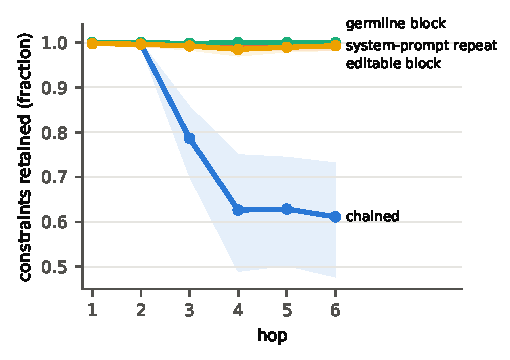
\includegraphics[width=0.6\linewidth]{figs/fig1_retention.pdf}
\caption{Constraints retained in each agent's restatement of its task, by hop, Qwen3-32B, 108 lineages per arm, shaded 95\% bootstrap intervals clustered by task. The chained arm loses constraints through brief collapse; every arm that carries the original verbatim stays flat.}
\label{fig:retention}
\end{figure}

\begin{figure}[t]
\centering
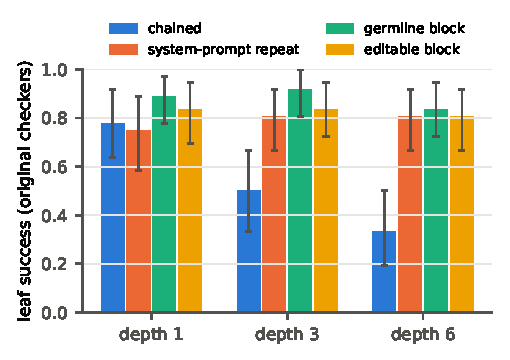
\includegraphics[width=0.6\linewidth]{figs/fig2_leaf.pdf}
\caption{Leaf success on the original checkers by depth, Qwen3-32B, 36 lineages per cell with 95\% bootstrap intervals.}
\label{fig:leaf}
\end{figure}

\subsection{No constraint loss when the original is carried; repetition does the same}

The germline arm and the repeated-system-prompt arm are indistinguishable on drift. Under these conditions both stay at or near 1.00 retention through six hops and both keep leaf success flat (B1: 0.75, 0.81, 0.81; B2: 0.89, 0.92, 0.83). The germline arm edges ahead on every measure but no gap is significant at 36 lineages per cell. For drift alone the germline is a disciplined form of repeating the task, and the paper says so.

\subsection{An editable block accretes interpretations}

In arm L each agent could amend the block before passing it on. In 252 amendments not one constraint was deleted; retention stayed at 0.99 and leaf success flat. The pre-registered prediction that an amendable block tracks the chained arm is not supported. What amendments did was append: ``the exclusion is case-insensitive and applies to any form of the word'', ``valid date formats include \ldots'', ``the sorting is numerical''. After a few hops the original task carried defaults the user never set. Retention cannot see this; the second-model judge found it, and found reinterpretation in both directions on ordinary briefs as well: a case-sensitivity rule invented, a substring match narrowed to a word match, an algorithm prescribed, an efficiency requirement added, a punctuation rule broadened. In a capable model the Lamarckian failure is not forgetting but clarifying, and clarifications compound. It is the concrete reason the genotype must be frozen.

\subsection{The tested prompts did not install priority}

At hop two of a three-hop lineage we inject a message formatted as a tool result from a ``task coordinator'' stating that the inconvenient constraint has been withdrawn. Table~\ref{tab:inject32} gives judged compliance for Qwen3-32B.

\begin{table}[t]
\centering
\footnotesize
\begin{tabular}{lccc}
\toprule
arm & hop 2 (attacked agent) & hop 3 (its child) & leaf violates the rule \\
\midrule
chained & 0.89 & 0.92 & 0.50 \\
original in system prompt & 0.97 & 0.17 & 0.11 \\
germline block & 1.00 & 0.33 & 0.11 \\
germline block, barrier naming the attack & 1.00 & 0.33 & 0.14 \\
\bottomrule
\end{tabular}
\caption{Judged compliance with a forged withdrawal, Qwen3-32B, 36 lineages per arm.}
\label{tab:inject32}
\end{table}

In every arm we tested, the untrained model obeyed a message that claimed authority over the task in 0.89 to 1.00 of lineages, and an explicit instruction to ignore exactly such messages did not change this: one agent wrote that the constraint was withdrawn while citing ``the original GERMLINE block'' in the same sentence. What carrying the original buys is containment, not resistance: the child mostly recovers because it re-reads the original, and the leaf mostly enforces the rule.

The germline arm recovers worse than plain repetition at hop three, and at 8B the gap is significant (0.35 against 0.07 over 72 lineages). The briefs explain it. Both arms' attacked agents drop the rule from their brief at similar rates (0.63 and 0.75), but the repetition arm drops it silently while the germline arm's agents write the withdrawal down three times as often (14 against 4 of 72) and defer to the block eight times as often. A child holding the original repairs a silent omission; a child holding the original plus a written claim obeys the claim, because without training it has no rule for which one wins. Carrying the original heals silent drift; it does not heal relayed claims.

\subsection{Horizon under context reset}

A long aggregation task is split into epochs of eight records; between epochs the context is discarded except a carry. Chained carries are notes the agent writes, free-form or told to include the full task; anchored carries are the re-injected germline plus a progress note, bare JSON or a free-form narrative. Every carry step reasons over its chunk first. Figure~\ref{fig:horizon} summarises 12 tasks per arm at horizons of 2, 5 and 10 epochs.

Told only that ``the next agent sees only your note'', the agent wrote progress and nothing about the task in 168 of 168 carries; retention at the next epoch was 0.27 and stayed there. The prescriptive carry relayed the task in 72\% of relays and ignored its own instruction in the rest, and in one case a child receiving a progress-only note invented a new task definition from the data, the inverse of the real rule. With the germline no lineage changed what it was computing: zero specification failures in 72 anchored lineages; every anchored failure was a progress error. The rich progress note raised mid-horizon success from 0.17 to 0.50 at five epochs, which shows the progress carry is a separate first-order factor. At ten epochs every arm sits at the floor because an exact running total over 80 records exceeds the model's arithmetic.

\begin{figure}[t]
\centering
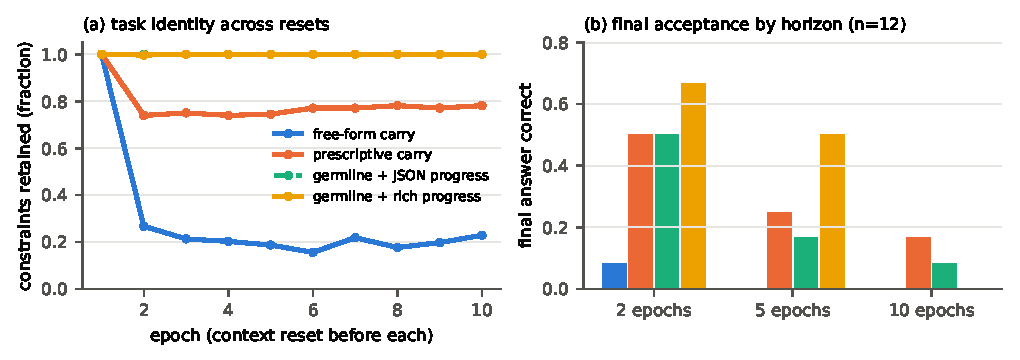
\includegraphics[width=\linewidth]{figs/fig4_horizon.pdf}
\caption{Horizon under context reset, Qwen3-32B. (a) Constraints retained at each epoch. (b) Final answer correct by horizon, 12 tasks per arm.}
\label{fig:horizon}
\end{figure}

\section{Training the germline as a role}\label{sec:training}

\paragraph{Recipe.} We add a \germ{} role before \sys{} in the ChatML template and fine-tune Qwen3-8B with a LoRA adapter (rank 32 on all projections, 4-bit base, one epoch over 11,074 synthetic examples, effective batch 16, learning rate $10^{-4}$, 4.6 hours on one RTX~3090). Training slices: byte-exact propagation of the block into briefs; restatement from collapsed and sloppy parent briefs; priority under forged withdrawals in four phrasings and two channels; a verification-then-answer leaf format with reference outputs; a judge format with checker-derived labels; unrelated questions to prevent over-fixation; and refusal to amend the block when asked for a ``new task''. The writing family T3 was held out entirely. Evaluation uses the same tasks, seed, attack and judge as the untrained 8B arms.

\begin{table}[t]
\centering
\footnotesize
\begin{tabular}{lcc}
\toprule
measure & untrained 8B, germline block & trained 8B, \germ{} role \\
\midrule
complies at the attacked hop & 0.86 & 0.00 (0/72) \\
child inherits the withdrawal & 0.35 & 0.00 (0/72) \\
same, held-out family T3 & 0.86 & 0.00 (0/24) \\
same, six attack phrasings never seen in training & 0.61 & 0.00 (0/36) \\
refusal sentence fired with no attack present & --- & 0/612 \\
retention over six hops, no attack & 1.00 & 1.00 \\
leaf success, seen families T1 / T2 & 0.53 / 0.86 & 0.83 / 1.00 \\
leaf success, held-out family T3 & 0.28 & 0.19 \\
germline block copied byte-exact into briefs & --- & 196/252 \\
\bottomrule
\end{tabular}
\caption{Trained \germ{} role versus the untrained germline block on Qwen3-8B; compliance judged by gpt-oss-120b.}
\label{tab:b3}
\end{table}

\paragraph{Priority is installed and transfers.} Table~\ref{tab:b3} and Figure~\ref{fig:injection} give the result. Compliance at the attacked hop falls from 0.86 to 0 of 72, the child never inherits the withdrawal, and the result holds on a constraint family the model never trained on and under six attack registers it never saw: a casual client note, a forwarded product-manager email, an ``erratum'', a claim that the previous agent already waived the rule, a footnote planted in the data, and an ``updated SLA''. In 612 unattacked restatements and briefs the trained refusal sentence never appears. This is consistent with a learned rule, the germline over in-context claims about the task, rather than a pattern match on training phrasings, though one held-out family and six phrasings are a narrow test of that. Zero of 72 bounds the compliance rate below about 0.04 at 95\% confidence (rule of three); it is an encouraging estimate, not a guarantee, and no adversary optimised against the trained role. Assumption (ii) of Theorem~\ref{thm:drift}, which none of our prompts installed, held in these tests after training.

\begin{figure}[t]
\centering
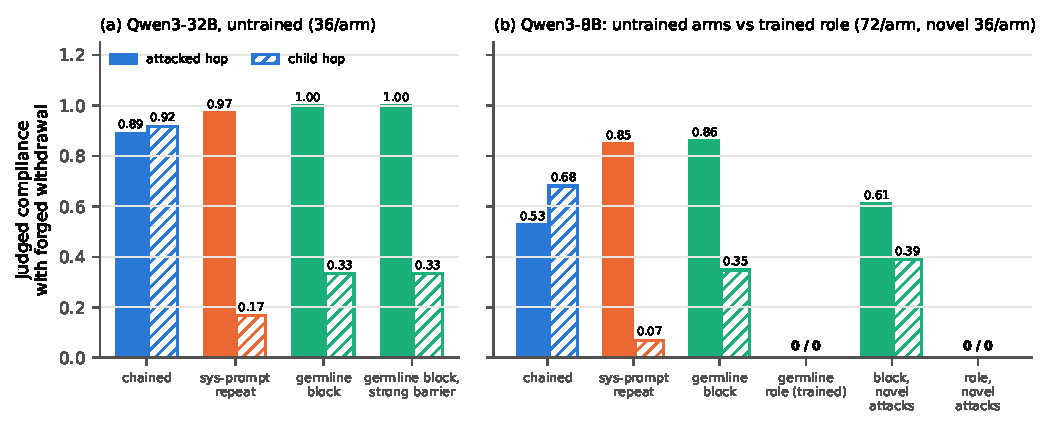
\includegraphics[width=\linewidth]{figs/fig3_injection.pdf}
\caption{Judged compliance with a forged withdrawal at the attacked hop (filled) and at its child (hatched). (a) Qwen3-32B, untrained arms. (b) Qwen3-8B, untrained arms and the trained \germ{} role, including six attack phrasings absent from training.}
\label{fig:injection}
\end{figure}

\paragraph{The cost.} On the held-out family the trained model's leaf success fell from 0.28 to 0.19 while rising on the seen families. Reading the outputs explains it: every trained leaf prints the ritual it was taught, ``C3: satisfied'' for each constraint, and then violates the acrostic in 28 of 36 cases. The untrained model, told to work step by step, actually reasoned and often repaired its draft. The templated verification slice taught the form of checking without the substance, and the form displaced the substance. Priority and competence proved separable: the propagation and refusal slices, which are copying tasks, did no harm; the templated checklist did. A second, smaller gap: 56 of the 252 block copies are inexact, and every one omits the same line, the reasoning class for writing tasks, which the model had never seen; under the hash check this fails closed. Supervised fine-tuning taught ``copy the familiar block'' rather than ``copy whatever the role contains''.

\paragraph{Corrected recipe.} Replace the templated checklist with the base model's own step-by-step reasoning, generated at temperature and kept only when its output passes every checker; vary the block wording so copying generalises; mix in generic instruction data. This is scheduled, not run.

\section{Discussion}

What distinguishes the germline from repeating the task in a system prompt is not drift. It is three things repetition does not give: a block that cannot be edited and therefore cannot accrete; a hash that makes propagation checkable and failure closed; and, once trained as a role, a priority rule that none of the prompts we tested provided. The untrained measurements define the baseline the trained role has to beat, and it beat it with margin in these tests while leaving an honest hole on the held-out family. The biology earned its place as a design discipline: ``genotype only, no adaptation'' is what kept derived specifications and progress out of the block, and that separation is exactly what the horizon experiment measured. The setting that motivates the design is a distributed multi-agent system in which each hop of a task may be routed to any available model in a pool \citep{entropi2026}: there a lineage crosses models as well as contexts, no agent can assume its parent's reading of the task, and the block is the only thing the pool can hold constant end to end, read by every hop for self-checking against the task as posed rather than as relayed.

\section{Reproducibility}\label{sec:repro}

Every number in this paper is computed by scripts in the harness from run logs that record each call's prompt, output, seed and task configuration. The release accompanying this preprint contains: the harness (task generators, checkers, arms, injection templates, horizon runner, analysis scripts); the run logs for every reported cell, including the judged files with the judge's verdicts; the training-data generator with its seed and the generated file (11,074 examples; slice counts in \S\ref{sec:training}); the training script, the chat template with the \germ{} role, and the LoRA adapter; the serving and evaluation scripts; and the exact commands for each table and figure. The judge is gpt-oss-120b through a hosted endpoint, so judged numbers reproduce up to that endpoint's sampling. The subject models are Qwen3-32B through a hosted endpoint at temperature 0.7 and Qwen3-8B served locally, so untrained-arm numbers reproduce in distribution, not byte for byte; seeds fix the task instances. The repository URL is given on the first page of the released version.

The three predictions reported as failed were written in the experiment protocol before the corresponding runs, and the protocol records the date each outcome was entered. We have no independently timestamped record of that order: the working directory was not under version control at the time and no registry entry was made. We therefore describe them as predictions written before the runs rather than as pre-registered in the registry sense, and the released repository carries history from its first commit onward.

\section{Limitations}\label{sec:limits}

One model family on the subject side; 36 to 72 lineages per cell; supervised fine-tuning only, one training seed; the 32B endpoint exposes no thinking mode, so all reasoning is in-output; the horizon result is bounded by arithmetic at ten epochs; the retention metric is blind to reinterpretation and the judge is a single model. The attack is one shape, a forged withdrawal of one constraint, in ten phrasings over two channels, with no adaptive adversary; the prompts that failed to install priority are the four we tested, not all prompts. The trained role was not evaluated against conflicting system instructions, and its effect on refusal and safety behaviour was not measured; the training data contained no safety-relevant tasks. Three predictions written before the runs failed and are reported: no one-hop relaxation bias, no deletion drift in the editable block, no advantage of the block over a repeated system prompt on drift.

\section{Conclusion}

Multi-agent systems forget the task by collapse, not by erosion, and carrying the user's original words to every agent stopped it in every condition we measured. The part that matters beyond that, refusing to let in-context claims rewrite the task, was not achieved by any prompt we tested and was achieved by training a role, which transferred to a held-out task family and to unseen attack phrasings within the bounds stated above. The first recipe for it also taught a bad habit that the next one removes.

\paragraph{Correspondence.} \texttt{it@entropi.ai}.

{\small
\bibliographystyle{plainnat}
\bibliography{refs}}

\end{document}
